%%%%%%%%%%%%%%%%%%%%%%%%%%%%%%%%%%%%%%%%%%%%%%%%%%%%%%%%%%%%%%%%%%%%%%%%%%%%%%%%%%%%
% Styles
%
% \textit{}
% \footnotemark~
% \footnotetext{}
% \url{}
% \textbf{}
% \noindent
% \begin{itemize}[nosep]
%		\item
% \end{itemize}
% \hyperlink{page.9}{page~9~(DSPL)}
%%%%%%%%%%%%%%%%%%%%%%%%%%%%%%%%%%%%%%%%%%%%%%%%%%%%%%%%%%%%%%%%%%%%%%%%%%%%%%%%%%%%

\documentclass[runningheads,a4paper]{llncs}
\usepackage{amssymb}
\setcounter{tocdepth}{3}
\usepackage{graphicx}
\usepackage{amssymb}
\usepackage{enumitem}
\usepackage[utf8]{inputenc}
\usepackage[hidelinks]{hyperref}
\usepackage{url}
\usepackage{float}
\usepackage{amsmath}
\usepackage{graphicx}
\usepackage{wrapfig}
\usepackage{fancyhdr}
\usepackage{titling}
\usepackage{xcolor}
\usepackage{lipsum}
\newcommand{\robospecs}{%
	\newpage%
	\pagenumbering{gobble}%
	\pagestyle{fancy}%
	\fancyhf{}%
	\rhead{$|$\footnotesize\thetitle}%
	\lhead{\footnotesize\theauthor }%
	\rfoot{Robot software and hardware specification sheet}%
}


%%%%%%%%%%%%%%%%%%%%%%%%%%%%%%%%%%%%%%%%%%%%%%%%%%%%%%%%%%%%%%%%%%%%%%%%%%%%%%%%%%%%
% Title
%
% Team Description Paper submitted for qualification in the 2020 RoboCup@Home international competition to be held in Bordeaux, France.
%%%%%%%%%%%%%%%%%%%%%%%%%%%%%%%%%%%%%%%%%%%%%%%%%%%%%%%%%%%%%%%%%%%%%%%%%%%%%%%%%%%%
\title{AZ5 2020 Team Description Paper}

\author{
  ................. ............. ..................
  \and ................. ............. ..................
  \and ................. ............. ..................
  \and ................ ................. ...........
}
\institute{Complubot, \\
\texttt{http://www.complubot.com/projects/az5/}}


\begin{document}
\maketitle

%%%%%%%%%%%%%%%%%%%%%%%%%%%%%%%%%%%%%%%%%%%%%%%%%%%%%%%%%%%%%%%%%%%%%%%%%%%%%%%%%%%%
% Abstract
%
%	Max: 250 word
% Paragraphs:
% - Introduction and relevance
% - Approach
% - Contributions
% Main research line, scientific achievements, problems solved and research group focus
% Approach to the problem solution and results expected to obtain
%%%%%%%%%%%%%%%%%%%%%%%%%%%%%%%%%%%%%%%%%%%%%%%%%%%%%%%%%%%%%%%%%%%%%%%%%%%%%%%%%%%%
\begin{abstract}
A custom made robotics platform that aims to be low cost, ROS compatible and suited for robotics researchers will be presented.
Currently it is used by the team to develop and test their algorithms.
Along the paper the focus will be on the software developed for the platform as well as the software developed.

The research line of the team is oriented to online object and person recognition, identification, tracking and reidentification.
To do so convolutional neural networks, feature extraction and feature matching, optical flow and color processing techniques are used.
The partial results of the different algorithms are combined with a kalman like filter to estimate the best action that the robot should perform to follow a selected target.
The target could be totally or partially occluded to the robot sight but it will keep tracking down the target even with slow rates of new images compared with the robot's control cycle rates. 

The researcher community has a great interest on these topics, specially on the robotics field.
It is our goal to contribute with a robotics platform that is capable of solving this tasks which are a solid base for other areas like person interaction or tridimensional recognition.
The platform will provide not only the hardware requirements to investigate in this fields but also our implementations to solve these problems.
\end{abstract}

%%%%%%%%%%%%%%%%%%%%%%%%%%%%%%%%%%%%%%%%%%%%%%%%%%%%%%%%%%%%%%%%%%%%%%%%%%%%%%%%%%%%
% Content
%
% Max: 8 pages
% Detailed information on the on the technical and scientific approach of the team's research.
% Current research, clearly stating all scientific contribution, and why are they important for you and the league
%%%%%%%%%%%%%%%%%%%%%%%%%%%%%%%%%%%%%%%%%%%%%%%%%%%%%%%%%%%%%%%%%%%%%%%%%%%%%%%%%%%%
\section{Introduction}
Our goal is to create an affordable and customizable platform suited for robotics researchers.
The platform is specially oriented to solve problems in the computer vision oriented towards robotics field.
The research team uses this platform to investigate in this fields so the platform keeps improving to fullfil their requirements.

This approach is quite different to the one that the software robotics community has.
We strongly believe that the hardware should adapt to the software researchers by providing them with what they need by been customizable and creating as less limitations as possible.

%%%%%%%%%%%%%%%%%%%%%%%%%%%%%%%%%%%%%%%%%%%%%%%%%%%%%%%%%%%%%%%%%%%%%%%%%%%%%%%%%%%%
% Robot description
%
% Unless your research revolves around hardware design and implementation, it is better to omit this section
% Avoid explaining ROS
% Keep it simple, more descriptive and less analytic.
% The main goal of a TDP is tell others about your latest practical achievement, what strategy was chosen and why, while at the same time trying to convince your reader that what you are doing is useful or applicable in a daily life scenario
%%%%%%%%%%%%%%%%%%%%%%%%%%%%%%%%%%%%%%%%%%%%%%%%%%%%%%%%%%%%%%%%%%%%%%%%%%%%%%%%%%%%
\subsection{Robot description}
The hardware and components details will be detailed in the annex, but the main ideas that had oriented the design of the platform will address here.
Our design is oriented to be suited for robots whose main focus is image capturing.

The robot has an omnidirectional motor platform with mecanum wheels.
It is capable to reach high speeds up to 1 meter per second but also to be able to move at slower but still controlled velocities.
These features are crucial to be able to follow a person that is moving at a normal indore speed.
With this type of motor platform the robot will be able to follow its target or even to walk along it.
This type of behavior is not often achievable with other motor platform on the market so there is not currently much research of this type of human-machine interaction.
Also mecanum wheels makes our platform capable of move a total of 50kg minus the platform's weight.

Motor platforms are usually closed without offering much room for hardware modifications.
Our approach is quite different and we spect the users of our platform to have the intention of adding new hardware to it.
With this in mind our platform is powered with a fully featured computer leaving room for another one.
The battery system is capable of maintaining both computers as well as the sensors and actuators providing extra outlets for more devices.
There is room to add cameras or other sensors to the platform and place them at a desired height.

%%%%%%%%%%%%%%%%%%%%%%%%%%%%%%%%%%%%%%%%%%%%%%%%%%%%%%%%%%%%%%%%%%%%%%%%%%%%%%%%%%%%
% Achievements
%
% One paragraph to summarize the experience and achievements of your team.
% The main focus should be on describing the solution and not the team.
%%%%%%%%%%%%%%%%%%%%%%%%%%%%%%%%%%%%%%%%%%%%%%%%%%%%%%%%%%%%%%%%%%%%%%%%%%%%%%%%%%%%
\subsection{Team achievements}



%%%%%%%%%%%%%%%%%%%%%%%%%%%%%%%%%%%%%%%%%%%%%%%%%%%%%%%%%%%%%%%%%%%%%%%%%%%%%%%%%%%%
% Content
%
% Innovative technology and scientific contribution
% Focus of research/research interests
% Re-usability of the system for other research groups
% Applicability of the robot in the real world
% When the robot depicted in the TDP or Team Video is different from the league's standard one, the TDP must clearly state how the addressed approach and described software will be adapted to the standard platform robot.
% Everything must be in perfect standard scientific English
%%%%%%%%%%%%%%%%%%%%%%%%%%%%%%%%%%%%%%%%%%%%%%%%%%%%%%%%%%%%%%%%%%%%%%%%%%%%%%%%%%%%
\section{Main research}
In this section the software created by the research team for the platform and in the field of robot computer vision will be presented.
The team has been two years working on the development of the platform so most of the work done has been oriented to this.

\subsection{Software for the platform}
Some sensors and actuators have been custom made.
In order to integrate them with the rest of the system we have made them ROS compatible.
\subsubsection{Sonar ring}
A ring with sixteen sonars is used to detect reflective objects.
This component is adapts to the sonar configuration and number.
The core of the component is platform independent so it can be run with different controllers if the sensor type is the same.
This component reads and filters the sensor data and publish it to ROS.

Using sonars works better to detect reflective objects than lidar does.
With different surfaces, specially dark or reflective ones lidar does not recognize them properly.
The sonars in contrast are capable of detecting them.

\subsubsection{Control platform}
Each of the four motors of the mecanum platform is controlled independently.
A hall sensor is used to calculate the speed of the wheel and classic control to controle it.
The architecture of the controllers is distributed trough i2c.

The master board can communicate through i2c and ROS.
It will receive velocities desired for the robot and transform them to velocities for the wheels.
Those velocities will then be sent to the slave boards.
This configuration allows high performance control over the wheels at a low cost.

\subsubsection{Bumpers}
Bumpers are used as an additional safety feature.
Their state is read and publish to ROS so safety actions can be performed.

\subsection{Online person recognition, identification, tracking and reidentification}
Our approach to perform this tasks makes use of varios simplifications of the problem to orient it towards mobile robotics.
Person recognition is achieved with Yolo-v3.
With it we can recognize where a person is.
That information is used to feed a Kalman like filter that uses a Markov grid with the resolution of the with of the image.

Person identification is achieved with hog feature description of the image [1] and which is used to feed a face landmark estimation algorithm[2].
Then the face landmarks are encoded so with this approach face recognition and face identification are possible.
The robot will take multiple image of its target and process them in order to get various encodings that are use to discriminate the targets face from other faces recognized on the image.
The position of the faces is also feed to the Kalman like filter.
With the face encodings we can differentiate between the target's face and other faces by calculating the distance between the two vectors.
Similar faces produce vectors that are closer than not so similar ones.

Additionally the color of the detected persons cloths is used to discriminate from one person to another.
This provides a fast but not as reliable way to identify the target.
This is needed because the face recognition algorithm can only work when the person is looking towards the robot.
With it the probability with which the target is detected when it is not looking at the robot is increased.

Finally to implement the prediction step on the Kalman like filter optical flow is used.
The optical flow is calculated for every person and face detected and the gaussian curves at those regions on the filter are relocated and stretched toward they have moved between the lasts frames.
This improves the tracking capabilities when the person is recognized between adjacent frames and hel us discriminate the target from other persons when they are group or walking together.

Tracking is achieved with the Kalman like filter.
The filter consist on a Markovian grid where gaussian curves are place with the image with resolution.
Then the grid is translated to an angle that indicates the angle between where the robot is facing and where the target is.
This angle is used by the robot to follow its target.

When the robot is close enough to the target it will stop moving.
At this point interaction between the robot and the target could begin.
If the target moves the robot will keep following him.

By processing the probability distribution on the Markov grid it is possible to infer if the target is being tracked correctly.
If the probability of the target position gets too low he is asked to be re recognized by the robot.
This is done by him standing in front of the robot for a small period of time.
During that time images will be taken to retrieve the color of the target's cloths as well as its facial encoding. 

%%%%%%%%%%%%%%%%%%%%%%%%%%%%%%%%%%%%%%%%%%%%%%%%%%%%%%%%%%%%%%%%%%%%%%%%%%%%%%%%%%%%
% Implemented algorithms transversal to the latest research that are also used
%%%%%%%%%%%%%%%%%%%%%%%%%%%%%%%%%%%%%%%%%%%%%%%%%%%%%%%%%%%%%%%%%%%%%%%%%%%%%%%%%%%%
\section{Robot capabilities}
The robot is able to navigate through the environment to specific locations safely.
The steps to do so goes as follows.

First we must create a map of the environment, which can be done by the robot itself without external aid.
The robot will wander through the environment using both sonars and lidar to avoid obstacles.
Meanwhile it will be mapping and localizing itself using a SLAM algorithm with the lidar data as input.

Once the map has been created we will be able to place metric goals over it.
The robot is able to go to each of them avoiding obstacles.
To calculate the path that the robot will follow we place random points over the map and link them together when they are linkable with an straight line.
The the shortest path though those links from the current position to the goal position is calculated.

This path is interpolated online to create an smooth output velocities that the robot will need to perform in order to reach the goals.
This velocities are not followed right away.
Instead a local planner based on VFH will correct them in order to avoid obstacles along the way.

This architecture can be used with different algorithms since its modular enough.
As an example to follow people with our online person recognition, identification, tracking and reidentification algorithm small steps where done.
First we needed to transform the output of the algorithm to an stearin direction that if the robot followed it would go after the target.
This stearin value was then provided as an input of the local planner.
Once this was done the robot was capable to follow its target as well as to avoid obstacles while doing so.

\section{Experiments and results}
Right now the robot is capable of tracking a person that is partially or totally occluded along different frames.
Te robot navigates towards its target avoiding obstacles and stops when it is near it.
At this point the robot will be ready to start interacting with with its target.

Also if the target has been for a long time not been captured by the robot, for example because it has been doing other tasks, it is capable of reidentificating it once it directly looks at the robot.

Our approach to identify persons is not to intrusive.
Also it allows to take on new targets quite easily.
Nevertheless the main problem of the current approach is that it offers very different results depending on the following factors.
When the person is looking directly at the robot the tracking capabilities improve greatly.
So in order to maintain high the level of confidence of our decisions we require for the target to look back to the robot from time to time.
Also drastic light changes affect the performance of the implementation, nevertheless this lose of confidence is detectable and we can ask the target to stop and let us re-learn its features in order to keep tracking it.

\section{Conclusions and future work}
We aim to develop the implementation of an online object and person recognition, identification, tracking and reidentification algorithm.
Our current approach makes a few simplifications to this general problem.
We want to keep improving our solution that currently is not capable of tracking multiple targets.
We also simplified the problem by just focussing on person tracking but we want to also address the problem of object tracking.
This two will be the main goals to focus on for the research team along the future years.

The robot is capable of capturing image depth.
On our current approach we are not taking advantage of this information but we are currently working on incorporate it on future versions of the implementation.
We are also not taking full advantage of having both a lidar and a sonar sensor.
This will be solved by using sensor mixing techniques with the camera lidar and sonars.
Combining both three sensors can improve greatly our obstacle detection capabilities like we can se on [2] detecting glass with sonars and on [3] improving thin objects detection. 

This part of the computer vision field has caught the attention of many researchers that are proposing different approaches to solve it.
The research team wants to create different implementations using this new ideas on the robot platform.
This will help to discover new ways to improve the platform as well as toto better understand the proposed solutions.
By doing so those implementations will be available to the ROS community.
Some of the implementations we want to bring to the ROS community are based on [5-7].
Those implementations are focussed on 3D person recognition and person reidentification using triplet loss.

The team wants to keep improving the platform so we are currently looking to compete with it in order to gain field experience and discover new challenges to overcome.
We hope to get in touch and compare ourselves with other teams in order to learn from ours and their mistakes.

%%%%%%%%%%%%%%%%%%%%%%%%%%%%%%%%%%%%%%%%%%%%%%%%%%%%%%%%%%%%%%%%%%%%%%%%%%%%%%%%%%%%
% Bibliography
%%%%%%%%%%%%%%%%%%%%%%%%%%%%%%%%%%%%%%%%%%%%%%%%%%%%%%%%%%%%%%%%%%%%%%%%%%%%%%%%%%%%
\newpage
\bibliographystyle{unsrt}
\bibliography{bibliography}

\newpage
\robospecs

%%%%%%%%%%%%%%%%%%%%%%%%%%%%%%%%%%%%%%%%%%%%%%%%%%%%%%%%%%%%%%%%%%%%%%%%%%%%%%%%%%%%
% OPL Annex
%
% Recommended 1 page
% The TDP's Robot Description Annex is an appendix of arbitrary length that must be attached at the end of the TDP and summarize the robot's software and hardware technical specifications.
% In this section briefly describe the software and hardware of the robot
%
% Purpose
% It allows the league to track changes in hardware and software trends over time.
% It helps experienced teams to find alternatives to their solutions when looking to improve or conducting benchmarking.
% It serves as a quick reference guide for new teams while preparing their robots.
%%%%%%%%%%%%%%%%%%%%%%%%%%%%%%%%%%%%%%%%%%%%%%%%%%%%%%%%%%%%%%%%%%%%%%%%%%%%%%%%%%%%

%%%%%%%%%%%%%%%%%%%%%%%%%%%%%%%%%%%%%%%%%%%%%%%%%%%%%%%%%%%%%%%%%%%%%%%%%%%%%%%%%%%%
% Parts of the robot
% Devices: bateries, motors, arms, cameras, lidar...
%%%%%%%%%%%%%%%%%%%%%%%%%%%%%%%%%%%%%%%%%%%%%%%%%%%%%%%%%%%%%%%%%%%%%%%%%%%%%%%%%%%%
\section*{Robot's Hardware Description}
\label{sec:annex-OPL}


%%%%%%%%%%%%%%%%%%%%%%%%%%%%%%%%%%%%%%%%%%%%%%%%%%%%%%%%%%%%%%%%%%%%%%%%%%%%%%%%%%%%
% Photo of the robot
%%%%%%%%%%%%%%%%%%%%%%%%%%%%%%%%%%%%%%%%%%%%%%%%%%%%%%%%%%%%%%%%%%%%%%%%%%%%%%%%%%%%
\setlength\intextsep{0pt}
\begin{wrapfigure}[10]{r}{0.3\textwidth}
	\centering
	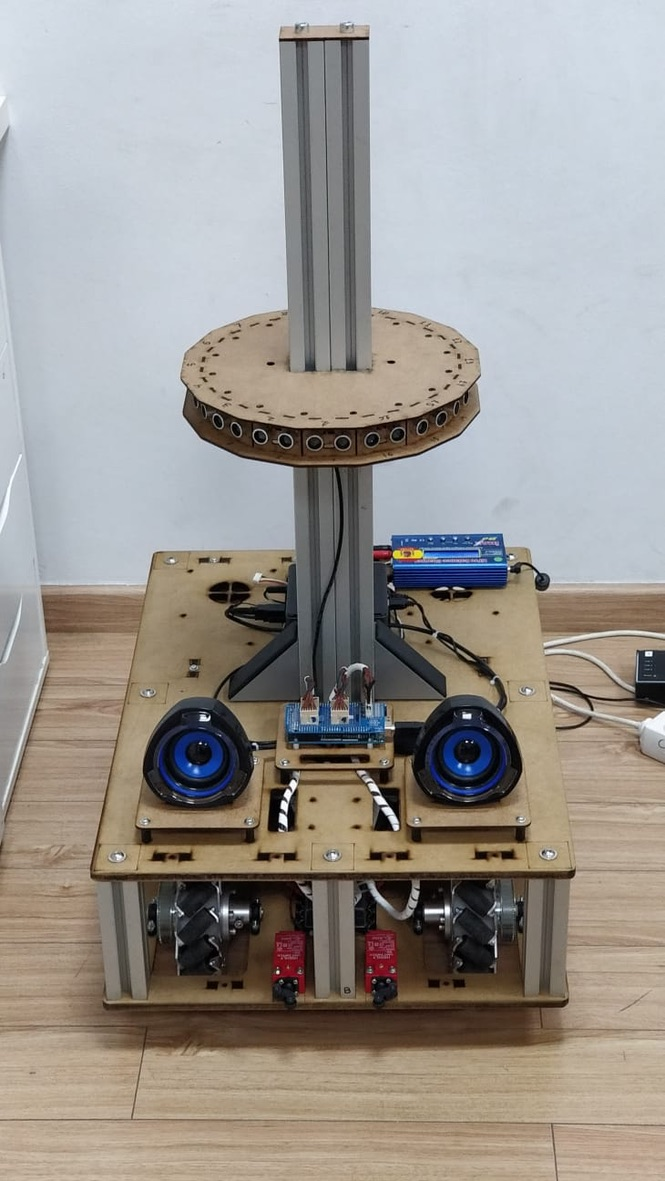
\includegraphics[width=0.4\textwidth]{images/AZ5.jpeg}
	\caption{AZ5}
	\label{fig:wall-e}
\end{wrapfigure}

%%%%%%%%%%%%%%%%%%%%%%%%%%%%%%%%%%%%%%%%%%%%%%%%%%%%%%%%%%%%%%%%%%%%%%%%%%%%%%%%%%%%
% Robot SW
% Platform:Operating System
% Navigation
% Recognition
% Speech recognition
% Speech generation
% Arms control...
%%%%%%%%%%%%%%%%%%%%%%%%%%%%%%%%%%%%%%%%%%%%%%%%%%%%%%%%%%%%%%%%%%%%%%%%%%%%%%%%%%%%
\section*{Robot's Software Description}



%%%%%%%%%%%%%%%%%%%%%%%%%%%%%%%%%%%%%%%%%%%%%%%%%%%%%%%%%%%%%%%%%%%%%%%%%%%%%%%%%%%%
% External devices
% 
% Cloud computing
% External computing or actuators
%%%%%%%%%%%%%%%%%%%%%%%%%%%%%%%%%%%%%%%%%%%%%%%%%%%%%%%%%%%%%%%%%%%%%%%%%%%%%%%%%%%%
\section*{External Devices}



%%%%%%%%%%%%%%%%%%%%%%%%%%%%%%%%%%%%%%%%%%%%%%%%%%%%%%%%%%%%%%%%%%%%%%%%%%%%%%%%%%%%
% SAS
%
% Geolocalization
% Language processing
%%%%%%%%%%%%%%%%%%%%%%%%%%%%%%%%%%%%%%%%%%%%%%%%%%%%%%%%%%%%%%%%%%%%%%%%%%%%%%%%%%%%
\section*{Cloud Services}

\nocite{*}
\end{document}
